\chapter{Common Startup Mistakes}

This chapter follows the final practical movement of MIT OpenCourseWare's \emph{Nuts and Bolts of New Ventures}, curated by LazyingArt LLC through Video2Book. The lecture is not a theory of startups in the abstract. It is Marina Hatzopoulos's deep-tech operating memory, framed by Bob Jones as part of a course whose speakers were ``well orchestrated, but not scripted.'' The point is that recurring warnings have independent empirical force. We will keep that rhythm: first the case, then the mechanism, then the practical rule.

\section{A Deep-Tech Case, Not a Startup Slogan}

Bob's handoff matters. Marina notices that some of her slides overlap with earlier speakers; Bob tells the class that the speakers did not coordinate their remarks. If the same patterns recur, the repetition is evidence. It says that entrepreneurs keep encountering the same traps.

Marina begins with her own path. She studied math and music, then went to banking, where she learned three business skills she later names explicitly: accounting, selling, and negotiation. At Thermo Electron, now Thermo Fisher, she discovered that evaluating a technology company was not just evaluating financial statements. It required judgment about the technology itself. That gap took her to MIT for a master's degree in mechanical engineering, not because she intended to become an engineer, but because she needed to manage engineers and speak their language.

The turning point was the Technology Licensing Office. MIT had patented inventions made by faculty and students, and the office looked for people and companies to commercialize them. In that setting Marina encountered an early 3D-printing technology, before ``3D printing'' had become a common term. The project had been led by Professor Ely Sachs, and two engineers had turned the printhead problem around: instead of designing a printhead for a material system, they designed a material system around an off-the-shelf inkjet printhead.

That reversal is already a deep-tech lesson. The invention was not merely an idea for a company. It was a technical possibility, protected by intellectual property, still searching for a product, a market, and a business.

Z Corporation was founded in 1994 in Kendall Square. The company delivered its first product within two years, reached profitability two years later, and eventually grew to about
\begin{equation}
\text{revenue}\approx \$30\text{M},\qquad
\text{employees}\approx 125,
\end{equation}
with no venture capital. Marina is careful about the interpretation: they did not avoid venture capital because they were cleverer than everyone else; nobody would invest in a hardware company at the moment when the Internet was taking off. That constraint became part of the company's discipline.

The lecture's first rough time scale is therefore not glamorous:
\begin{equation}
\text{deep-tech venture horizon}\sim 10\ \text{years}.
\end{equation}
For deep tech, this is not a warning meant to discourage us. It is a boundary condition. If we build the chapter correctly, the later advice about patents, prototypes, customers, price, cash, and board-level decisions all has to fit inside this long clock.

\section{Intellectual Property and Proof of Principle}

Marina next asks why someone creates a startup. The motives can differ: passion for a technology, desire to solve a problem, independence, teamwork, community, or money. Her point is not that one motive is nobler than another. It is that the founder has to know the motive, because the definition of success depends on it. A founder trying to diagnose brain tumors may make different business choices from a founder trying to maximize personal financial return.

Then she narrows the frame: for a deep-tech startup, the starting point should be intellectual property. A patent is presented as a bargain. We disclose how to do something, and in exchange receive a time-limited monopoly:
\begin{equation}
\text{patent protection}\approx 20\ \text{years}.
\end{equation}
This is not merely legal ornament. In Z Corporation's case, Marina says a large customer took apart their machine, but did not enter with a competitive product until after the MIT patents expired. The patent period bought the company time to invest, educate the market, and grow.

The order of disclosure is equally important. For researchers and graduate students, publication brings credibility, but the lecture's rule is:
\begin{equation}
\text{patent first}\quad\longrightarrow\quad \text{publish second}.
\end{equation}
Once the work is published, Marina says, the opportunity to patent can be lost. The statement should be preserved as a practical warning from the lecture, not expanded into a complete legal doctrine. The legal mechanism is more nuanced in the real world, but the operating rule for the founder in the lecture is clear: do not publish away the boundary that protects the venture.

The second technical object is the proof of principle. Marina distinguishes it from a finished product. The early machine was ugly. It required people to stand over it and pour powder. It used multiple computers. But it proved that a paper-printer-derived process could build a three-dimensional part. In our notation:
\begin{equation}
\text{proof of principle}
\neq
\text{finished product},
\qquad
\text{proof of principle}\Rightarrow
\text{core technical risk reduced}.
\end{equation}

\begin{remark}
In this lecture, intellectual property is the North Star. When the market is unclear, when customers disagree, and when the team does not know which path to follow, Marina repeatedly returns to the question: what makes us special that we can protect?
\end{remark}

\section{From Stealth to Market Disruption}

One early mistake is part-time entrepreneurship. Marina accepts Bob's earlier qualification: one should validate before quitting a job. But once the venture is validated and moving forward, time matters. A startup done for a few hours on Saturday morning is not likely to move fast enough. Researchers need entrepreneurs, and entrepreneurs need researchers.

She then turns to another founder instinct: staying stealth. Founders often fear that if they share the idea, someone will steal it. Marina's correction is sharper: if all we have is an idea, then anyone can copy it once it reaches the market anyway. The right protection is not silence about the problem. It is a combination of patents, trade secrets, know-how, and disciplined judgment about what not to reveal.

Customers do not need to know the inner workings. They need to know whether we solve their problem. The questions are:
\begin{equation}
\text{painful problem?}\qquad
\text{large enough market?}\qquad
\text{worth entering?}
\end{equation}

\begin{figure}
\centering

\includegraphics[width=\linewidth]{lecture_10_figure_02.png}
\caption{Market disruption sources. The slide supplies the categories; the photograph is illustrative.}
\end{figure}

The slide gives the compact set of disruption sources:
\begin{equation}
D\in\{\text{regulations},\ \text{demographic changes},\ \text{new enabling technologies}\}.
\end{equation}
The transcript adds the caution that not all disruptions last long enough to support a company. Marina gives examples of transient openings: corporate investment in DEI initiatives, and many companies built around temporary COVID problems. The relevant test is duration:
\begin{equation}
\text{startup opportunity}
\approx
\text{disruption with enough duration for company formation}.
\end{equation}

\subsection{Question \& Answer}

Why does disruption help a startup, when large companies have almost every advantage?

Large companies have manufacturing, research and development, sales, marketing, distribution, money, experience, market knowledge, customer relationships, and brands. Marina says they have absolutely everything except the ability to pivot quickly. The startup edge is not that incumbents are stupid. The edge is maneuverability:
\begin{equation}
\text{startup edge}
=
\text{ability to pivot under incomplete information}.
\end{equation}
The more innovative the market, the less complete the information. A startup is therefore not solving a well-posed problem set. It is learning in fog. New information has to change direction.

\section{Market and Technology Development Interact}

The next move is the lecture's main formal model. In deep tech, two paths must be developed at the same time. One path is technical: run tests, try different technology directions, de-risk the highest-risk elements, and avoid building the entire system before learning whether a subcomponent works. The other path is market-facing: articulate the technology advantage, consider many industries, speak with experts, test possible markets quickly, and talk to customers.

The transcript gives a rough target:
\begin{equation}
N_{\text{market ideas}}\approx 20.
\end{equation}
This is not a statistical sample size. It is a practical antidote to premature narrowing. Marina calls the early market search speed dating, not dinner. We are looking for fast disconfirmation and promising signals.

\begin{figure}
\centering

\includegraphics[width=\linewidth]{lecture_10_figure_03.png}
\caption{Market and technology iteration. The slide's arrow is informal; it marks a feedback loop, not a theorem.}
\end{figure}

The slide states the relation in ordinary slide notation:
\begin{equation}
\text{iterative process}\Rightarrow
\text{information from one drives the other}.
\end{equation}
For notes, the clean reconstruction is:
\begin{equation}
\text{market learning}\longleftrightarrow \text{technology development}.
\end{equation}

\begin{figure}
\centering
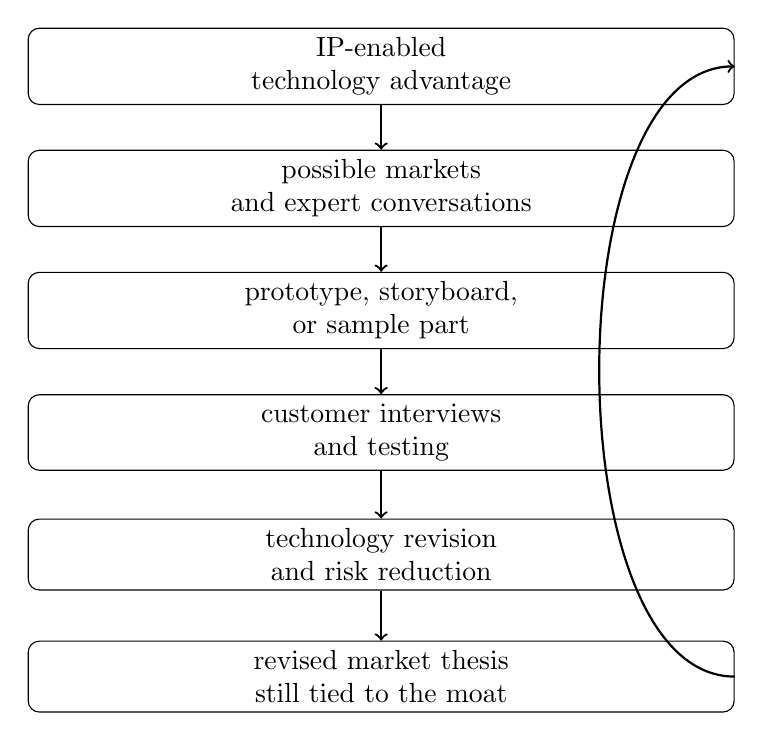
\begin{tikzpicture}[
  box/.style={draw, rounded corners, align=center, text width=0.72\linewidth, minimum height=0.9cm},
  arr/.style={->, thick}
]
\node[box] (ip) at (0,0) {IP-enabled\\technology advantage};
\node[box] (markets) at (0,-1.55) {possible markets\\and expert conversations};
\node[box] (proto) at (0,-3.10) {prototype, storyboard,\\or sample part};
\node[box] (test) at (0,-4.65) {customer interviews\\and testing};
\node[box] (revise) at (0,-6.20) {technology revision\\and risk reduction};
\node[box] (thesis) at (0,-7.75) {revised market thesis\\still tied to the moat};

\draw[arr] (ip) -- (markets);
\draw[arr] (markets) -- (proto);
\draw[arr] (proto) -- (test);
\draw[arr] (test) -- (revise);
\draw[arr] (revise) -- (thesis);
\draw[arr] (thesis.east) .. controls (2.2,-7.75) and (2.2,0) .. (ip.east);
\end{tikzpicture}
\caption{A pocket-safe reconstruction of the deep-tech feedback loop. Product-market fit is useful only if it remains connected to protectable differentiation.}
\end{figure}

\subsection{Question \& Answer}

How do we validate a deep-tech idea before there is a finished product?

Marina's answer is to move in stages. First build a proof of principle to remove the core technical risk. Then build a crude prototype, storyboard, or sample part to communicate with customers. The artifact need not be beautiful. It has to be concrete enough that customers can react to it.

The validation update rule is:
\begin{equation}
\text{crude artifact}
\longrightarrow
\text{customer feedback}
\longrightarrow
\text{technical revision}
\longrightarrow
\text{better artifact}.
\end{equation}
In the Z Corporation story, she took sample parts to a trade show without even having a booth. Many customers criticized the part quality. She answered with speed: they could have a part quickly rather than waiting until tomorrow. That imperfect feedback still revealed where the technology might matter.

The general rule is an evidence gradient:
\begin{align}
\text{compliment} &< \text{reaction to idea} \\
&< \text{reaction to prototype} \\
&< \text{near-real product use} \\
&< \text{customer money}.
\end{align}
The closer the customer is to using the actual product as intended, the more useful the feedback becomes.

\section{Differentiation, Customers, and the Pricing Pivot}

The lecture now enters its repeated pattern: mistake, then correction. One mistake is to seek a popular market because everyone is talking about it. The crowded market looks promising; the founder imagines there is room for another Pepsi beside Coke; the founder assumes incumbents are slow and stupid; the founder believes price can be lowered if needed.

Marina rejects that logic. Lowering price is not the answer. In deep tech, the state of the art is the starting point, not the endpoint. The aim is to do something so much better on a dimension the customer cares about that the product can command a premium:
\begin{equation}
\text{protectable differentiation}
\quad\Rightarrow\quad
\text{possible premium price}.
\end{equation}

Competition is more subtle. For Z Corporation, competition from other non-giant 3D-printing firms helped educate the market. Once customers understood why they might need a 3D printer, Z Corporation could sell against alternatives by showing where it was faster, cheaper, or capable of color. The worst competitor was not always another machine. Sometimes it was doing nothing.

The central quantitative story begins with the initial market. High-end rapid-prototyping machines sold for approximately
\begin{equation}
\$100{,}000\ \text{to}\ >\$1{,}000{,}000.
\end{equation}
Z Corporation planned to enter at the low end with an office-compatible machine:
\begin{equation}
P_0=\$20{,}000.
\end{equation}
A year into development, before launch, the two incumbents announced office-compatible machines at
\begin{equation}
P_{\text{incumbent}}=\$60{,}000.
\end{equation}
At the trade show, Z Corporation learned that its technology was about
\begin{equation}
\text{speed advantage}\approx 10\times
\end{equation}
faster than the incumbent technologies, even though its parts had shortcomings. That evidence changed the decision. Walter Bornhorst, the chairman, proposed matching the competitor's price:
\begin{equation}
\$20{,}000\longrightarrow \$60{,}000.
\end{equation}

\subsection{A Worked Decision Update}

We can write the pricing story as a simple update, not as a universal formula. Let \(P\) be the contemplated product price, and let \(E\) be the new evidence learned before launch:
\begin{equation}
E=
\{\text{incumbents at } \$60{,}000,\ 
\text{Z Corp speed}\approx 10\times,\ 
\text{customers care about speed}\}.
\end{equation}
The original plan was
\begin{equation}
P_{\text{old}}=\$20{,}000.
\end{equation}
The update was
\begin{equation}
P_{\text{new}}
=
\operatorname{revise}(P_{\text{old}}\mid E)
=
\$60{,}000.
\end{equation}
The decision did not say, ``always triple price.'' It said: when the evidence changes the customer's value perception and the product has not yet launched, remake the strategic decision. Marina adds a practical asymmetry:
\begin{equation}
\text{lowering price after launch is easier than raising price after launch}.
\end{equation}
The higher price turned out to matter because production, sales, and market education were more expensive than expected. Educating the market took about one year from introduction to purchase:
\begin{equation}
\text{market-education cycle}\approx 1\ \text{year}.
\end{equation}

\subsection{Question \& Answer}

When should we listen to customers, and when should we ignore them?

Marina does not give a magic rule. She says entrepreneurship constantly involves listening and not listening. Customers may dismiss the new thing because they cannot yet imagine it. Industry veterans may say the idea is stupid. But the farther the conversation is from actual product use, the weaker the feedback. The closer the feedback is to the intended use of a real product, the stronger it becomes.

There is also a danger on the other side: power users can pull the company into a narrow, expensive direction. Z Corporation built a larger machine because a significant fraction of early customers asked for one. In hindsight, the market was limited and the technical challenges were larger than expected. The project pulled against the long-term path of making the machine less expensive and easier to use. The test is therefore:
\begin{equation}
\text{customer request useful?}
\quad\Longleftrightarrow\quad
\text{request lies on the long-term strategic path}.
\end{equation}

\section{Teams, Conflict, and Strategic Decisions}

The next mistakes are internal. Hiring people one trusts sounds reasonable, but loyal friends and family may not supply the missing skills. A famous board chair who is too busy may be less useful than a less famous person who is engaged. Z Corporation's founding team mattered because it had complementary capabilities: business strategy, business execution, material science, software, and hardware.

The lecture's team rule can be stated as:
\begin{equation}
\text{founding strength}
\approx
\text{complementary skills}
+
\text{mutual respect}
+
\text{ability to make hard changes}.
\end{equation}
Marina adds a practical warning: do not hire someone you cannot fire. If possible, work with someone before hiring them. A one-week trial can reveal more than an interview.

The cultural mistake is to be merely nice. Marina distinguishes courtesy from avoidance. Z Corporation argued about everything, but without grudges. The argument was productive because each person came from a different perspective. In business terms:
\begin{equation}
\text{diverse views}+\text{nonpersonal conflict}
\longrightarrow
\text{better decisions}.
\end{equation}

The next trap is confusing work volume with strategic work. A founder can generate enormous satisfaction by checking off easy items, but the company needs the number one item, not the seventeenth. Marina separates strategic and non-strategic decisions:
\begin{align}
\text{strategic} &=
\{\text{business},\ \text{team},\ \text{product},\ \text{pricing}\},\\
\text{non-strategic} &=
\{\text{offices},\ \text{furniture},\ \text{software choice},\ \text{conference rooms}\}.
\end{align}
The strategic decisions should be revisited when new information arrives:
\begin{equation}
\text{new information}
\quad\Rightarrow\quad
\text{remake strategic decisions}.
\end{equation}

No venture capital was not originally a chosen strategy for Z Corporation, but it had strategic consequences. The company had to bootstrap, reach revenue quickly, and focus on profitability. Marina summarizes the scale as:
\begin{equation}
\text{capital}\approx \$2.5\text{M},
\qquad
\text{revenue}\approx \$30\text{M}.
\end{equation}
Again, this is case data, not a benchmark. The lesson is not that every company should avoid venture capital. The lesson is that financing constraints shape operating discipline.

\section{Pitching, Funding, and Venture Capital}

Investor communication is another place where founders put on a show. Marina warns against acronyms that outsiders do not know, complicated diagrams, paragraphs in tiny fonts, hockey-stick projections, exit talk in the pitch, confidentiality demands, and adding AI no matter what business one is in. The correction is simplification.

\begin{figure}
\centering

\includegraphics[width=\linewidth]{lecture_10_figure_04.png}
\caption{Simplifying the investor pitch. The slide includes the visible presentation guideline of roughly 10--20 words per slide.}
\end{figure}

The visible guideline is:
\begin{equation}
\text{words per slide}\sim 10\text{--}20.
\end{equation}
The spoken pitch template is:
\begin{equation}
\text{We make \underline{\hspace{1.5cm}} for \underline{\hspace{1.5cm}} to \underline{\hspace{1.5cm}}.}
\end{equation}
The blanks are product, customer, and problem. If the listener does not know what the product is, who the customer is, and what problem is being solved, the technical detail will not rescue the pitch.

Marina then widens the funding map. Friends and family are often first. Angels can range roughly from
\begin{equation}
\$25{,}000\ \text{to}\ \$1{,}000{,}000.
\end{equation}
Government grants can matter greatly in deep tech. Strategic investors can include suppliers, customers, and distributors. R\&D contracts are non-dilutive and validating. Customer deposits can also fund operations:
\begin{equation}
\text{deposit}=20\%,
\qquad
\text{delivery}\approx 3\text{--}6\ \text{months}.
\end{equation}
Venture capital and venture debt enter the map, but not as the universal destination.

\subsection{Question \& Answer}

Is venture capital always the right path?

No. Marina gives both sides. Venture capital can provide cash, advice, connections, and validation. Some businesses need it: a two-sided global market like Uber, or a capital-heavy satellite company, may require large and fast financing.

But venture capital also carries risks. With too much money, a company may move forward without product-market fit. Some markets cannot grow at the pace venture investors expect. Founders can lose control. A high valuation raises the bar for investor returns. The more precise comparison is:
\begin{equation}
\text{founder outcome}
\neq
\text{headline valuation}.
\end{equation}
Marina's example is intentionally concrete: a very profitable \(\$10\text{M}\) company that the founder owns entirely may be better for that founder than pushing toward a billion-dollar outcome and failing. The correct financing path depends on the business.

Fundraising itself is work. Research investors before pitching them. If an investor only funds AI software and the company is a 3D-printer company, do not pitch and call it optimism. Marina's blunt rule is to reject yourself before collecting needless rejection. Each failed pitch should produce a strategic takeaway:
\begin{equation}
\text{failed pitch}
\longrightarrow
\{\text{wrong investor},\ \text{unclear pitch},\ \text{flawed business model}\}.
\end{equation}

\section{CEO Syndrome and Course Closure}

The last founder mistake is psychological. Early CEOs are challenged constantly by engineers, customers, investors, and employees. That challenge forces rework: redesign the product, redefine product-market fit, and sharpen the value proposition. Then success arrives. People begin to call the CEO a visionary. Awards and visibility accumulate. New employees never saw the early uncertainty. The CEO starts to feel invincible.

The danger is a feedback loop in which success destroys the very challenge that produced success.

\begin{figure}
\centering
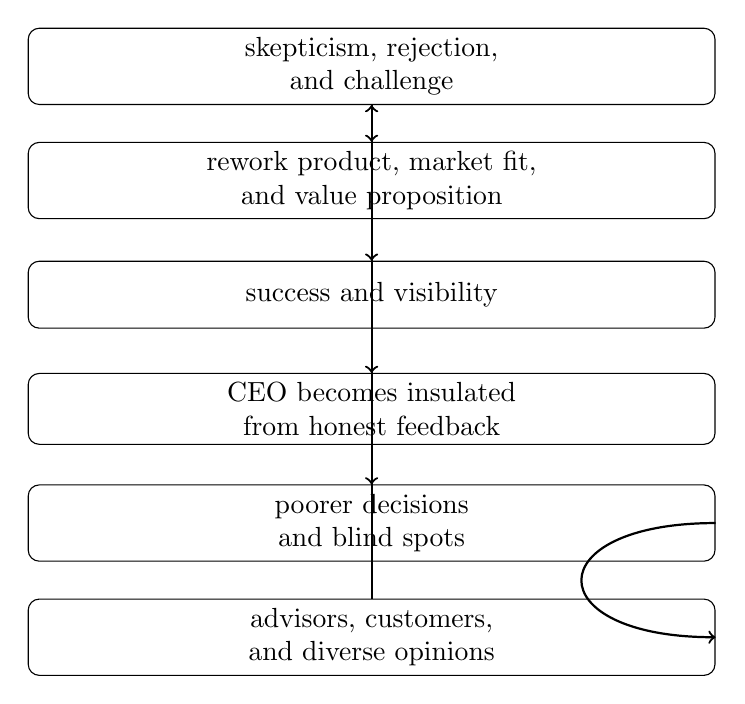
\begin{tikzpicture}[
  box/.style={draw, rounded corners, align=center, text width=0.70\linewidth, minimum height=0.85cm},
  arr/.style={->, thick}
]
\node[box] (challenge) at (0,0) {skepticism, rejection,\\and challenge};
\node[box] (rework) at (0,-1.45) {rework product, market fit,\\and value proposition};
\node[box] (success) at (0,-2.90) {success and visibility};
\node[box] (insulate) at (0,-4.35) {CEO becomes insulated\\from honest feedback};
\node[box] (bad) at (0,-5.80) {poorer decisions\\and blind spots};
\node[box] (advisors) at (0,-7.25) {advisors, customers,\\and diverse opinions};

\draw[arr] (challenge) -- (rework);
\draw[arr] (rework) -- (success);
\draw[arr] (success) -- (insulate);
\draw[arr] (insulate) -- (bad);
\draw[arr] (advisors) -- (challenge);
\draw[arr] (bad.east) .. controls (2.1,-5.80) and (2.1,-7.25) .. (advisors.east);
\end{tikzpicture}
\caption{A conceptual reconstruction of CEO syndrome and its antidote. The challenge loop must be deliberately restored.}
\end{figure}

The antidote is not humility as a slogan. It is structure: an advisory group willing to challenge ideas, customers close enough to use the product, and an organization that asks questions and listens. Small failures and small rejections feel unpleasant, but they are the mechanism that improves decisions.

Marina closes by restating the essentials for deep-tech hardware: defensible product differentiation, a strong and diverse team, debate and healthy culture, customer contact, prototype use, revenue and profitability in the beachhead market, and decisions remade whenever new information arrives.

Bob then returns to the course as a whole. The course was not meant to be theory; it was meant to increase the probability of success. Entrepreneurship is called a full-contact sport, not an academic exercise. The closing slide points students toward MIT's entrepreneurship resources.

\begin{figure}
\centering

\includegraphics[width=\linewidth]{lecture_10_figure_05.png}
\caption{MIT entrepreneurship roadmap. The detailed logos are best preserved as screenshot evidence rather than redrawn.}
\end{figure}

The visible roadmap carries participation counts:
\begin{equation}
50{,}000+,\quad 5{,}000+,\quad 2{,}000+,\quad 350,\quad 72.
\end{equation}
In the chapter, the important content is not the small logos but the direction: inspiration, exploration, fundamentals, application, and acceleration. Bob also names the Venture Mentoring Service as a place where entrepreneurs receive homework, mentor teams, and repeated meetings.

The final formula is Joseph Hadzima's course heuristic:
\begin{equation}
H=\frac{R}{E}.
\end{equation}
Happiness \(H\) rises when reality \(R\) exceeds expectations \(E\). Bob's closing interpretation is practical: in everything we do, ask whether we can create a reality that exceeds the expectations people have. That is a fitting end to a course about startups because the same fraction governs customers, investors, employees, and founders themselves.

\section{Summary}

The lecture begins with a case and ends with a course-wide rule. In between, Marina's argument is consistent: deep-tech entrepreneurship starts with protectable differentiation, then tests market reality without giving away the core secret. We should expect fog, incomplete information, and wrong turns. The work is to build enough proof to learn, enough customer contact to steer, enough team conflict to decide well, and enough financial discipline to survive.

The central update is the Z Corporation pricing decision:
\begin{equation}
(\$20{,}000,\ \text{low-end entry})
\quad\stackrel{\text{new evidence}}{\longrightarrow}\quad
(\$60{,}000,\ \text{premium speed value}).
\end{equation}
That is the lecture in miniature. A startup is not a fixed plan. It is a protected technical possibility learning its way through the market.